\section{Lecture 3}

\subsection{Volume conservation in the phase space} 
It is crucial that the algorithm is time-reversible (if we start from $B^{*}$, we arrive exactly on $A^{*}$), and that the volume in the phase space is not compressed (\textit{i.e.} that the volume is conserved).
We are going to explain this very important point thanks to some graphical examples.

    \begin{figure}[H]
        \centering
        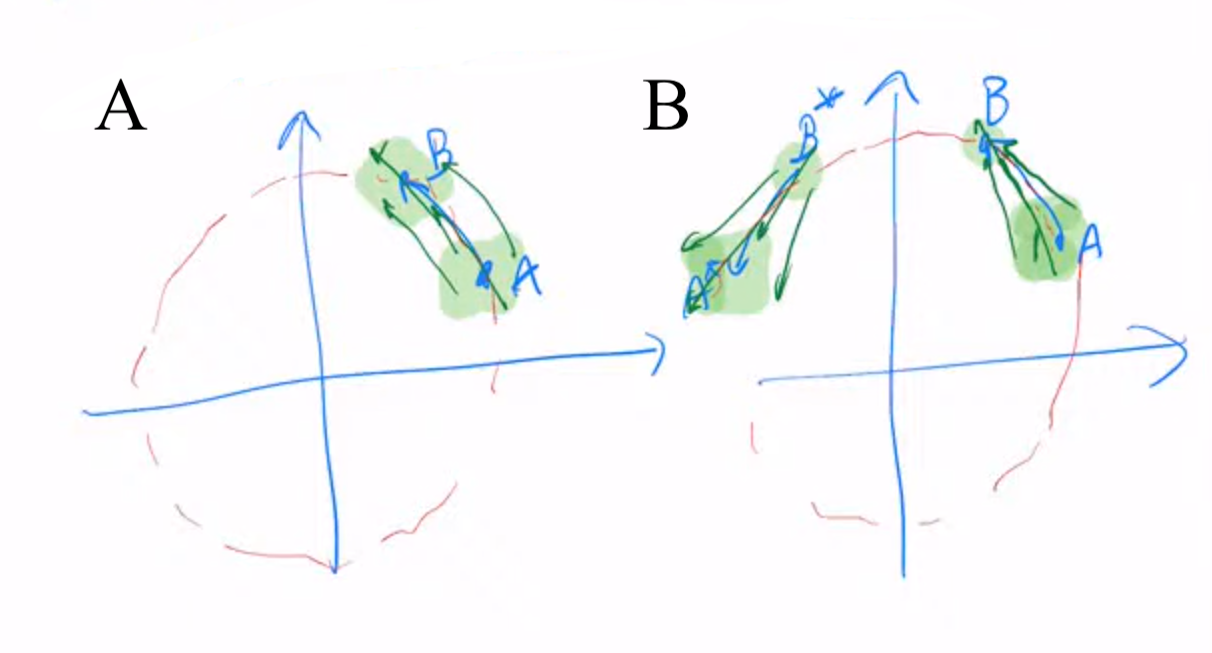
\includegraphics[width=0.9\textwidth]{Monte Carlo/images/lect3/graphex}
        \caption{Graphical explanation for the volume conservation}
        \label{fig:verlet_freepart}
    \end{figure}

\noindent \textbf{A:} Here, the differential equation brings the system from $A$ to $B$ exactly, and this is also true for multiple copies of the system that occupy the area in green. Here, the volume (in the phase space) is preserved because the group of replicates of the system ends up on a new position which occupies the exact same volume. We can also say that density in the phase space is conserved.\\
\textbf{B:} In the second example, the differential equation does not conserve the volume in the phase space. Indeed, it brings the replicates of the system from $A$ to $B$, but the area it occupied in $A$ is not the same one that it occupies in $B$. \\ 
Notice that until now, we only used algorithms that preserve the volume in the phase space (Taylor and Trotter expansion). In order to see "what not to do", here is an algorithm which exactly conserves the energy but does not conserve the volume in the phase space. 

\begin{algorithm}[H]
			\caption{Example of an algorithm that does not conserve the volume}
			\begin{algorithmic}[0]
				\For{i in range(...)}
				    \State $E_{0}$= U(q) + K(p)
					\State p += f/2*$\Delta$t
					\State q+=p/m*$\Delta$t
					\State f=force(q)
					\State 	p+=f/2*$\Delta$t 
					\State $E_{1}$= U(q) + K(p)
					\State p *= $\sqrt{((K+E_{0}-E_{1})/K)}$
				\EndFor
			\end{algorithmic}
\end{algorithm}
The goal of this algorithm is to show how to create an algorithm that does not conserve the volume in the phase space. In order to do this, we first used Velocity-Verlet algorithm. Remember: Velocity-Verlet is time reversible, preserves the volume in the phase space, but violates the conservation of the energy. This violation means that after the velocities and coordinates are modified, the energy changes. \\
We wanted an algorithm that conserves the energy, so at line 7, we rescaled all the velocities with the factor $\sqrt{\frac{K+E_{0}-E_{1}}{K}}$ in order to compensate the error made with Velocity-Verlet algorithm. After this modification of the velocities (and thus, of the kinetic energy), the energy is exactly equal to $E_{0}$. \\
Therefore, the energy is exactly conserved : this algorithm will generate structures that have exactly the same energy but there is not guarantee that they are taken from the microcanonical ensemble (it is very difficult to know how far they are taken from it). As we increase the time-step, states continue to have the same energy but the distribution becomes incorrect. And this very last point means that our algorithm does not conserve the volume in the phase space, because the distribution of the states in the phase space is not conserved. \\

\subsection{Hybrid Monte-Carlo}

Let's go back to Monte-Carlo. One could use a Monte-Carlo algorithm where instead of moving randomly positions and velocities, we move them by solving the Hamilton equations. More explicitly, we propose the moves by solving the Hamilton equations. If we solve Hamilton equations exactly, the energy will be exactly conserved and if Detailed-Balance is someway satisfied, the acceptance will always be equal to 1. In other words, all the moves will be accepted: it will be a very efficient algorithm. \\
Unfortunately, it is impossible to solve Hamilton equations exactly. We can only do it approximately, thanks for example to Velocity-Verlet algorithm. As we just saw, Velocity-Verlet algorithm is time-reversible, preserves the volume in the phase space but does not conserve the energy. Thus, we only have to include in the acceptance the violation in the energy conservation.
Such an algorithm is called Hybrid Monte Carlo (\href{https://www.sciencedirect.com/science/article/abs/pii/037026938791197X?}{\emph{see this paper}}).

\begin{algorithm}[H]
			\caption{Hybrid Monte-Carlo}
			\begin{algorithmic}[0]
				\For{istep in range(...)}
				    \State $E_{0}$= U(q) + K(p)
				    \State $p_{0}$=p
				    \State $q_{0}$=q
				    \For{i in range(nsteps)}
				        \State p += f/2*$\Delta$t
				        \State q += p/m*$\Delta$t
				        \State f = force(q)
				        \State p += f/2*$\Delta$t
				    \EndFor
					\State $E_{1}$= U(q) + K(p)
					\State $\alpha$ = min(1,$\exp(-\beta * E_{1}-E_{0})$)
					\If{$\alpha$ $>$ rand(0,1)}
					    \State pass
				    \Else
				        \State p=$p_{0}$    
				        \State q=$q_{0}$ 
				    \EndIf
				\State print(q,p)    
				\EndFor
			\end{algorithmic}
		\end{algorithm}
Notice that if we choose a very small $\Delta$t, energy will be conserved and then, we accept all the steps. If $\Delta$t is very large, most of the steps will be rejected.\\
Let’s say that one step is rejected. Then we try again starting from the same position and velocity. The algorithm is deterministic, so we end up with the same acceptance : we try and try again until the move is accepted. The important thing is that all the rejected moves will count when we will compute the averages.\\
This is not the best strategy. Typically people use this algorithm instead, by randomizing the velocities from a Boltzmann distribution, which corresponds to nothing more than a Gaussian distribution with 0 average and standard deviation equal to $\sqrt{m K_{B}T}$.
\begin{algorithm}[H]
			\caption{Better hybrid Monte-Carlo}
			\begin{algorithmic}[0]
				\For{istep in range(...)}
				    \State $E_{0}$= U(q) + K(p)
				    \State $p_{0}$=p
				    \State $q_{0}$=q
				    \State p = random.gauss(0,$\sqrt{(m K_{B}T}$)
				    \For{i in range(nsteps)}
				        \State p += f/2*dt
				        \State q += p/m*$\Delta$t
				        \State f = force(q)
				        \State p += f/2*$\Delta$t
				    \EndFor
					\State $E_{1}$= U(q) + K(p)
					\State $\alpha$ = min(1,$\exp(-\beta * E_{1}-E_{0})$)
					\If{$\alpha$ $>$ rand(0,1)}
					    pass
				    \Else
				        \State p=$p_{0}$    
				        \State q=$q_{0}$  
				    \EndIf
				\State print(q,p)    
				\EndFor
			\end{algorithmic}
		\end{algorithm}